\chapter{\sffamily Simple state transitions}

{\bfseries\sffamily Concept.} To define and develop an archetype simulation environment for simple state transitions. In our classification scheme, this archetype is defined by a trivial state partition graph topology and would make sense for simulations of sequential design problems, sports matches and other simple gameplay domains. We will also discuss the typical ways in which the state of the system may only partially be observed in realistic examples, and analyse how best to deal with each situation. For the mathematically-inclined, this chapter will define the mapping of our formalism to simple state transitions. For the programmers, the software which is designed and described in this chapter can be found in the public Git respository here: \href{https://github.com/worldsoop/worldsoop}{https://github.com/worldsoop/worldsoop}.


\section{\sffamily Defining the archetype}

The simple state transition archetype refers to simulation environments where there is no obvious computational benefit to partitioning the state into concurrently updating or acting on separate components. There may even be performance benefits from keeping state information all within the same common data structure in memory, but this can depend on the specific problem of study. In the interest of completeness with respect to the chapters which follow on from this one, we have illustrated the trivial state partition graph topology for this archetype in Fig.~\ref{fig:state-partition-graph-simple-state-transitions}.

\begin{figure}[h]
\centering
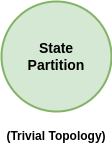
\includegraphics[width=2cm]{images/chapter-6-state-partition-graph.drawio.png}
\caption{State partition graph topology for simple state transition archetypes.}
\label{fig:state-partition-graph-simple-state-transitions}
\end{figure}

In order to understand what sorts of data might be collected about this archetype in realistic scenarios, let's begin by considering the types of real-world problem domain which could potentially leverage simulation environments to train control algorithms. The subset of these which may best suit the simple state transition environment archetype are:
%%
\begin{itemize}
\item{Event-based simulations of sports matches, e.g., football~\cite{pulis2022reinforcement}, rugby~\cite{sawczuk2022markov}, tennis~\cite{ding2022deep}, etc., and other forms of game --- all of which typically define a relatively simple global match/gameplay context as their `state'.}
\item{Sequential design simulations to change the configuration or data collection strategies of, e.g., astronomical telescopes~\cite{jia2023observation,yatawatta2021deep}, biological experiments~\cite{treloar2022deep} and user interfaces~\cite{lomas2016interface}, which typically define a relatively simple and finite set of possible actions that can be taken.}
\end{itemize}
%%
